\documentclass[12pt]{beamer}
\usepackage{../Estilos/BeamerFC}
\usepackage{../Estilos/ColoresLatex}
\usepackage{courier}
\usepackage{listingsutf8}
\usepackage{listings}
\usepackage{xcolor}
\usepackage{textcomp}
\usepackage{color}
\definecolor{deepblue}{rgb}{0,0,0.5}
\definecolor{brown}{rgb}{0.59, 0.29, 0.0}
\definecolor{OliveGreen}{rgb}{0,0.25,0}
% \usepackage{minted}

\DeclareCaptionFont{white}{\color{white}}
\DeclareCaptionFormat{listing}{\colorbox{gray}{\parbox{0.98\textwidth}{#1#2#3}}}
\captionsetup[lstlisting]{format=listing,labelfont=white,textfont=white}
\renewcommand{\lstlistingname}{Código}


\definecolor{Code}{rgb}{0,0,0}
\definecolor{Keywords}{rgb}{255,0,0}
\definecolor{Strings}{rgb}{255,0,255}
\definecolor{Comments}{rgb}{0,0,255}
\definecolor{Numbers}{rgb}{255,128,0}

\makeatletter

\newif\iffirstchar\firstchartrue
\newif\ifstartedbyadigit
\newif\ifprecededbyequalsign

\newcommand\processletter
{%
  \ifnum\lst@mode=\lst@Pmode%
    \iffirstchar%
        \global\startedbyadigitfalse%
      \fi
      \global\firstcharfalse%
    \fi
}

\newcommand\processdigit
{%
  \ifnum\lst@mode=\lst@Pmode%
      \iffirstchar%
        \global\startedbyadigittrue%
      \fi
      \global\firstcharfalse%
  \fi
}

\lst@AddToHook{OutputOther}%
{%
  \lst@IfLastOtherOneOf{=}
    {\global\precededbyequalsigntrue}
    {}%
}

\lst@AddToHook{Output}%
{%
  \ifprecededbyequalsign%
      \ifstartedbyadigit%
        \def\lst@thestyle{\color{orange}}%
      \fi
    \fi
  \global\firstchartrue%
  \global\startedbyadigitfalse%
  \global\precededbyequalsignfalse%
}

\lstset{ 
language=Python,                % choose the language of the code
basicstyle=\footnotesize\ttfamily,       % the size of the fonts that are used for the code
numbers=left,                   % where to put the line-numbers
numberstyle=\scriptsize,      % the size of the fonts that are used for the line-numbers
stepnumber=1,                   % the step between two line-numbers. If it is 1 each line will be numbered
numbersep=5pt,                  % how far the line-numbers are from the code
backgroundcolor=\color{white},  % choose the background color. You must add \usepackage{color}
showspaces=false,               % show spaces adding particular underscores
showstringspaces=false,         % underline spaces within strings
showtabs=false,                 % show tabs within strings adding particular underscores
frame=single,   		% adds a frame around the code
tabsize=2,  		% sets default tabsize to 2 spaces
captionpos=t,   		% sets the caption-position to bottom
breaklines=true,    	% sets automatic line breaking
breakatwhitespace=false,    % sets if automatic breaks should only happen at whitespace
escapeinside={| |},  % if you want to add a comment within your code
stringstyle =\color{OliveGreen},
otherkeywords={as, np.array, np.concatenate, np.linspace, linspace, interpolate.interp1d, kind, plt.plot, .copy, np.arange, np.cos, np.pi, lw, ls, label, splrep, splev, plt.legend, loc, plt.title, plt.ylim, plt.show, sign, math.ceil, math.log, np.sqrt, np.exp, np.zeros, plt.xlabel, plt.ylabel, plt.xlim, np.identity, random, np.dot, np.outer, np.diagonal },             % Add keywords here
keywordstyle = \color{blue},
commentstyle = \color{darkcerulean},
identifierstyle = \color{black},
literate=%
         {á}{{\'a}}1
         {é}{{\'e}}1
         {í}{{\'i}}1
         {ó}{{\'o}}1
         {ú}{{\'u}}1
%
%keywordstyle=\ttb\color{deepblue}
%fancyvrb = true,
}

\lstdefinestyle{FormattedNumber}{%
    literate={0}{{\textcolor{red}{0}}}{1}%
             {1}{{\textcolor{red}{1}}}{1}%
             {2}{{\textcolor{red}{2}}}{1}%
             {3}{{\textcolor{red}{3}}}{1}%
             {4}{{\textcolor{red}{4}}}{1}%
             {5}{{\textcolor{red}{5}}}{1}%
             {6}{{\textcolor{red}{6}}}{1}%
             {7}{{\textcolor{red}{7}}}{1}%
             {8}{{\textcolor{red}{8}}}{1}%
             {9}{{\textcolor{red}{9}}}{1}%
             {.0}{{\textcolor{red}{.0}}}{2}% Following is to ensure that only periods
             {.1}{{\textcolor{red}{.1}}}{2}% followed by a digit are changed.
             {.2}{{\textcolor{red}{.2}}}{2}%
             {.3}{{\textcolor{red}{.3}}}{2}%
             {.4}{{\textcolor{red}{.4}}}{2}%
             {.5}{{\textcolor{red}{.5}}}{2}%
             {.6}{{\textcolor{red}{.6}}}{2}%
             {.7}{{\textcolor{red}{.7}}}{2}%
             {.8}{{\textcolor{red}{.8}}}{2}%
             {.9}{{\textcolor{red}{.9}}}{2}%
             {\ }{{ }}{1}% handle the space
         ,%
          %mathescape=true
          escapeinside={__}
          }



\usetheme{Dresden}
\usecolortheme{seahorse}
%\useoutertheme{default}
\setbeamercovered{invisible}
% or whatever (possibly just delete it)
\setbeamertemplate{section in toc}[sections numbered]
\setbeamertemplate{subsection in toc}[subsections numbered]
\setbeamertemplate{subsection in toc}{\leavevmode\leftskip=3.2em\rlap{\hskip-2em\inserttocsectionnumber.\inserttocsubsectionnumber}\inserttocsubsection\par}
\setbeamercolor{section in toc}{fg=blue}
\setbeamercolor{subsection in toc}{fg=blue}
\setbeamercolor{frametitle}{fg=blue}
\setbeamertemplate{caption}[numbered]

\setbeamertemplate{footline}
\beamertemplatenavigationsymbolsempty
\setbeamertemplate{headline}{}

\makeatletter
\setbeamercolor{section in foot}{bg=gray!30, fg=black!90!orange}
\setbeamercolor{subsection in foot}{bg=blue!30!yellow, fg=red}
\setbeamertemplate{footline}
{
  \leavevmode%
  \hbox{%
  \begin{beamercolorbox}[wd=.333333\paperwidth,ht=2.25ex,dp=1ex,center]{section in foot}%
    \usebeamerfont{section in foot} \insertsection
  \end{beamercolorbox}}%
  \begin{beamercolorbox}[wd=.333333\paperwidth,ht=2.25ex,dp=1ex,center]{subsection in foot}%
    \usebeamerfont{subsection in foot}  \insertsubsection
  \end{beamercolorbox}%
  \begin{beamercolorbox}[wd=.333333\paperwidth,ht=2.25ex,dp=1ex,right]{date in head/foot}%
    \usebeamerfont{date in head/foot} \insertshortdate{} \hspace*{2em}
    \insertframenumber{} / \inserttotalframenumber \hspace*{2ex} 
  \end{beamercolorbox}}%
  \vskip0pt%
\makeatother 

\makeatletter
\patchcmd{\beamer@sectionintoc}{\vskip1.5em}{\vskip0.8em}{}{}
\makeatother

\usefonttheme{serif}

\title{\large{Cálculo de raíces}}
\subtitle{Tema 2 - Operaciones matemáticas básicas}
\author{M. en C. Gustavo Contreras Mayén}
\date{}

\begin{document}
\maketitle

\section*{Contenido}
\frame{\tableofcontents[currentsection, hideallsubsections]}

\section{Método de bisección}
\frame{\tableofcontents[currentsection, hideothersubsections]}
\subsection{La variable \texttt{switch}}

% % \begin{frame}[fragile]
% % \frametitle{Algoritmo para el método de bisección}
% % 	\begin{lstlisting}
% %     for i in np.arange(n):
% %         x3 = 0.5*(x1 + x2); f3 = f(x3)
% %         if (switch == 0) and (abs(f3) > abs(f1)) \
% %                         and (abs(f3) > abs(f2)):
% %             return None
% %         if f3 == 0.0: return x3
% %         if f2*f3 < 0.0:
% %             x1 = x3; f1 = f3
% %         else:
% %             x2 =x3; f2 = f3
% %     return (x1 + x2)/2.0
% % 	\end{lstlisting}

% % \end{frame}
% % \begin{frame}
% % Haciendo que la variable \texttt{switch} = 1, se forza la rutina para comprobar si la magnitud de $f(x)$ disminuye con la reducción a la mitad de cada intervalo.
% % \end{frame}
% % \begin{frame}
% % Si no es así, algo anda mal (probablemente la \enquote{raíz} no es una raíz en absoluto, sino una singularidad) y se devuelve la \texttt{raíz} = \texttt{None}.
% % \\
% % \bigskip
% % Dado que esta característica no siempre es deseable, el valor predeterminado es \texttt{switch}=0.
% % \end{frame}

\begin{frame}
\frametitle{Revisión de la variable}
Veamos lo que hace la variable \texttt{switch}:
\\
\bigskip
\pause
Hasta el momento no nos hemos fijado en la magnitud de $f (x_{1})$ y $f (x_{2})$, sólo y en el signo del respectivo producto, pero ahora, tomamos en cuenta la magnitud tanto de los puntos evaluados en la función como del producto mismo.
\end{frame}
\begin{frame}
\frametitle{Revisión de la variable}
Del ejercicio:
\begin{align*}
x^{3} - 10 \; x^{2} + 5 = 0
\end{align*}
\pause
Sabemos que hay una raíz en el intervalo $[0.6, 0.8]$
\end{frame}
\begin{frame}
\frametitle{Valores en una tabla}
\begin{table}
\centering
\renewcommand{\arraystretch}{0.9}
\begin{tabular}{c | c | c | c | c | c }
$x_{1}$ & $x_{3}$ & $x_{2}$ & $f (x_{1})$ & $f (x_{3})$ & $f (x_{2})$ \\ \hline
$0.00000$ & $0.50000$ & $1.00000$ & $5.00000$ & $2.62500$	& $-4.00000$ \\ \hline
$0.50000$ & $0.75000$ & $1.00000$ & $2.62500$ & $-0.20312$	& $-4.00000$ \\ \hline
$0.50000$ & $0.62500$ & $0.75000$ & $2.62500$ & $1.33789$	& $-0.20312$ \\ \hline
$0.62500$ & $0.68750$ & $0.75000$ & $1.33789$ & $0.59839$	& $-0.20312$ \\ \hline
% $0.68750$ & $0.71875$ & $0.75000$ & $0.59839$ & $0.20529$	& $-0.20312$ \\ \hline
% $0.71875$ & $0.73438$ & $0.75000$ & $0.20529$ & $0.00299$	& $-0.20312$ \\ \hline
% $0.73438$ & $0.74219$ & $0.75000$ & $0.00299$ & $-0.09959$	& $-0.20312$ \\ \hline
% $0.73438$ & $0.73828$ & $0.74219$ & $0.00299$ & $-0.04819$	& $-0.09959$ \\ \hline
% $0.73438$ & $0.73633$ & $0.73828$ & $0.00299$ & $-0.02257$	& $-0.04819$ \\ \hline
% $0.73438$ & $0.73535$ & $0.73633$ & $0.00299$ & $-0.00978$	& $-0.02257$ \\ \hline
% $0.73438$ & $0.73486$ & $0.73535$ & $0.00299$ & $-0.00340$	& $-0.00978$ \\ \hline
% $0.73438$ & $0.73462$ & $0.73486$ & $0.00299$ & $-0.00020$	& $-0.00340$ \\ \hline
% $0.73438$ & $0.73450$ & $0.73462$ & $0.00299$ & $0.00139$	& $-0.00020$ \\ \hline
% $0.73450$ & $0.73456$ & $0.73462$ & $0.00139$ & $0.00059$	& $-0.00020$ \\ \hline
\end{tabular}
\end{table}
\begin{tikzpicture}[overlay]
    \uncover<1>{\draw[thick, red] (0, 2.5) rectangle (11.3, 3.3);}
    \uncover<2>{\draw[thick, blue, fill=blue, opacity=0.2] (7.4, 2.5) rectangle (11.3, 3.3);}
    \uncover<3>{\draw[thick, blue, fill=blue, opacity=0.2] (5.5, 1.8) rectangle (9.3, 2.4);}
    \uncover<4>{\draw[thick, blue, fill=blue, opacity=0.2] (7.4, 1.1) rectangle (11.3, 1.7);}
    \uncover<5>{\draw[thick, blue, fill=blue, opacity=0.2] (7.4, 0.3) rectangle (11.3, 1);}
\end{tikzpicture}
\end{frame}
\begin{frame}
\frametitle{Valores en una tabla}
\begin{table}
\centering
\renewcommand{\arraystretch}{0.9}
\begin{tabular}{c | c | c | c | c | c }
$x_{1}$ & $x_{3}$ & $x_{2}$ & $f (x_{1})$ & $f (x_{3})$ & $f (x_{2})$ \\ \hline
% $0.00000$ & $0.50000$ & $1.00000$ & $5.00000$ & $2.62500$	& $-4.00000$ \\ \hline
% $0.50000$ & $0.75000$ & $1.00000$ & $2.62500$ & $-0.20312$	& $-4.00000$ \\ \hline
% $0.50000$ & $0.62500$ & $0.75000$ & $2.62500$ & $1.33789$	& $-0.20312$ \\ \hline
% $0.62500$ & $0.68750$ & $0.75000$ & $1.33789$ & $0.59839$	& $-0.20312$ \\ \hline
% $0.68750$ & $0.71875$ & $0.75000$ & $0.59839$ & $0.20529$	& $-0.20312$ \\ \hline
% $0.71875$ & $0.73438$ & $0.75000$ & $0.20529$ & $0.00299$	& $-0.20312$ \\ \hline
% $0.73438$ & $0.74219$ & $0.75000$ & $0.00299$ & $-0.09959$	& $-0.20312$ \\ \hline
% $0.73438$ & $0.73828$ & $0.74219$ & $0.00299$ & $-0.04819$	& $-0.09959$ \\ \hline
% $0.73438$ & $0.73633$ & $0.73828$ & $0.00299$ & $-0.02257$	& $-0.04819$ \\ \hline
\ldots & \ldots & \ldots & \ldots & \ldots & \ldots \\ \hline 
$0.73438$ & $0.73535$ & $0.73633$ & $0.00299$ & $-0.00978$	& $-0.02257$ \\ \hline
$0.73438$ & $0.73486$ & $0.73535$ & $0.00299$ & $-0.00340$	& $-0.00978$ \\ \hline
$0.73438$ & $0.73462$ & $0.73486$ & $0.00299$ & $-0.00020$	& $-0.00340$ \\ \hline
$0.73438$ & $0.73450$ & $0.73462$ & $0.00299$ & $0.00139$	& $-0.00020$ \\ \hline
$0.73450$ & $0.73456$ & $0.73462$ & $0.00139$ & $0.00059$	& $-0.00020$ \\ \hline
\end{tabular}
\end{table}
\begin{tikzpicture}[overlay]
    \uncover<1>{\draw[thick, red] (0, 3.3) rectangle (11.3, 3.9);}
    \uncover<2>{\draw[thick, blue, fill=blue, opacity=0.2] (5.5, 3.3) rectangle (9.3, 3.9);}
    \uncover<3>{\draw[thick, blue, fill=blue, opacity=0.2] (5.5, 2.5) rectangle (9.3, 3.1);}
    \uncover<4>{\draw[thick, blue, fill=blue, opacity=0.2] (5.5, 1.8) rectangle (9.3, 2.3);}
    \uncover<5>{\draw[thick, blue, fill=blue, opacity=0.2] (5.5, 1.1) rectangle (9.3, 1.6);}
    \uncover<6>{\draw[thick, blue, fill=blue, opacity=0.2] (5.5, 0.4) rectangle (9.3, 1.0);}
\end{tikzpicture}
\end{frame}
    
% \begin{frame}[fragile]
% \frametitle{Revisando el código}
% Del código tenemos que:
% \pause
% \begin{verbatim}
% if (switch == 0) and (abs(f3) > abs(f1)) \ 
%                  and (abs(f3) > abs(f2)):
%     return None
% \end{verbatim}
% \end{frame}
% \begin{frame}[fragile]
% \frametitle{Valor de la expresión}
% \begin{table}
% \centering
% \renewcommand{\arraystretch}{0.9}
% \begin{tabular}{l | l | l | l | c}
% $x_{1}$ & $x_{2}$ & $f(x_{1})$ & $f(x_{2})$ & $f (x_{1}) f (x_{2})$ \\ \hline
% $0.0$ & $0.2$ & $5.0$ & $4.608$ & $23.04$ \\ \hline
% $0.2$ & $0.4$ & $4.608$ & $3.464$ & $15.9621$ \\ \hline
% \end{tabular}
% \end{table}    

% \begin{table}
%     \centering  
% \begin{tabular}{l  | l | l}
% $\abs{f3} > \abs{f1}$ & $\abs{f3} > \abs{f2}$ & Expresión \\ \hline
% \texttt{True} & \texttt{True} & True \\ \hline
% \end{tabular}
% \end{table}

% \begin{tikzpicture}[overlay]
%     \draw[thick, red] (1.7, 6) rectangle (9.5, 7);
% \end{tikzpicture}
% \end{frame}

\section{Método de Newton-Raphson}
\frame{\tableofcontents[currentsection, hideothersubsections]}
\subsection{Definición}

\begin{frame}
\frametitle{Método de Newton-Raphson}
El método de Newton-Raphson es el algoritmo más conocido para encontrar raíces por una buena razón: es simple y rápido.
\\
\bigskip
\pause
El único detalle es que utiliza la derivada $\pderivada{f} (x)$ así como la función $ f(x)$. \pause Por tanto, en los problemas a resolver con este algoritmo, deberá de contemplarse que la derivada sea fácil de calcularse.
\end{frame}
\begin{frame}
\frametitle{Método de Newton-Raphson}
El método de Newton-Raphson (\funcionazul{MNR} se obtiene de la expansión en series de Taylor de $f (x)$ alrededor de $x$:
\pause
\begin{align*}
f (x_{i + 1})  = f (x_{i}) + \pderivada{f} (x_{i})(x_{i + 1} - x_{i}) +\order{x_{i + 1} - x_{i}}^{2}
\end{align*}
\end{frame}
\begin{frame}\frametitle{Método de Newton-Raphson}
Si $x_{i + 1}$ es una raíz de $f (x) = 0$, tenemos que:
\pause
\begin{align*}
0 = f (x_{i}) + \pderivada{f} (x_{i})(x_{i + 1} - x_{i}) + \order{x_{i + 1} - x_{i}}^{2}
\end{align*}
\pause
Suponiendo que $x_{i}$ está cerca de $x_{i + 1}$, podemos eliminar el último término de la ecuación y resolver para $x_{i+1}$, por lo que la fórmula de Newton-Raphson es:
\pause
\begin{align*}
x_{i+1} = x_{i} - \dfrac{f(x_{i})}{\pderivada{f} (x_{i})}
\end{align*}
\end{frame}
\begin{frame}
\frametitle{Error en el método}
Si $x$ representa el valor verdadero de la raíz, el error en $x_{i}$ es $E_{i} = x - x_{i}$.
\\
\bigskip
\pause
Se puede demostrar que si $x_{i+1}$ se calcula de la expresión del \funcionazul{MNR}, el error es:
\pause
\begin{align*}
E_{i+1} = - \dfrac{\sderivada{f} (x_{i})}{2 \, \pderivada{f} (x_{i})} \; E_{i}^{2}
\end{align*}
Lo que nos dice que el \funcionazul{MNR} converge de manera cuadrática, es decir, el error es el cuadrado del error del punto previo.
\end{frame}
\begin{frame}[fragile]
\frametitle{Representación gráfica}
Podemos interpretar que $x_{i+1}$ es el punto en donde la tangente de $f (x_{i})$ cruza el eje de las $x$:
\pause
\begin{center}
	\begin{tikzpicture}[font=\small, scale=0.8]
		\draw [->] (0,0) -- (7,0);
		\draw [<->] (0,-3) -- (0,3);
		\draw [red, thick] (1,3) .. controls (1.5,0.5) and (5,-2) .. (6.5,-2);
		\draw (1,-0.3) node {$x_{i}$};
		\draw (1,3.3) node {$f(x_{i})$};
		\draw [dashed] (1.2,0) -- (1.2,2.35);
		\draw (0.8,3.1) -- (2.35,-0.1);
		\draw [dashed] (2.3,0) -- (2.3,0.58);
		\draw (2.3,-0.3) node {$x_{i+1}$};
	\end{tikzpicture}
\end{center}
\end{frame}
\begin{frame}[fragile]
\frametitle{Criterio de convergencia}
El \funcionazul{MNR}, es sencillo: \pause se aplica la expresión para $x_{i + 1}$ iniciando con un valor $x_{0}$, hasta alcanzar un criterio de convergencia:
\pause
\begin{align*}
\abs{ x_{i+1} - x_{i} } < \varepsilon
\end{align*}
\end{frame}
\begin{frame}[fragile]
\frametitle{Algoritmo del método}
El algoritmo es el siguiente:
\pause
\setbeamercolor{item projected}{bg=lava,fg=white}
\setbeamertemplate{enumerate items}{%
\usebeamercolor[bg]{item projected}%
\raisebox{1.5pt}{\colorbox{bg}{\color{fg}\footnotesize\insertenumlabel}}%
}
\begin{enumerate}[<+->]
\item Sea $x$ un valor inicial para la raíz de $f (x) = 0$.
\item Calcular $\Delta x = - f (x)/\pderivada{f} (x)$.
\item Asignar $x \leftarrow x + \Delta x$ y se repiten los pasos 2-3, hasta alcanzar $\abs{ \Delta x } < \varepsilon$.
\end{enumerate}
\end{frame}
\begin{frame}[fragile]
\frametitle{Precaución con el \funcionazul{MNR}}
Aunque el \funcionazul{MNR} converge rápidamente cerca de la raíz, sus características globales de convergencia son pobres. 
\\
\bigskip
\pause
La razón es que la línea tangente no es siempre una aproximación aceptable de la función.
\end{frame}
\begin{frame}[fragile]
\frametitle{Precaución con el \funcionazul{MNR}}
\begin{center}
	\begin{tikzpicture}[font=\small, scale=0.8]
		\draw [->] (0,0) -- (4,0);
		\draw [<->] (0,-1) -- (0,3);
		\draw [red, thick] (1,3) .. controls (2,3) and (2.5,2) .. (3.5,-2);
		\draw (4.2,0) node {$x$};
		\draw (-0.5,2) node {$f (x)$};
		\draw (1.2,-0.2) node {$x_{0}$}; \pause
        \draw [fill=blue] (1.2,3) circle (0.05); \pause
        \draw [dashed] (1.2,0) -- (1.2,3); \pause
	    \draw [blue, ->] (1.2,3) -- (3.5,2.7);
	\end{tikzpicture}
\end{center}
\end{frame}
\begin{frame}[fragile]
\frametitle{Precaución con el \funcionazul{MNR}}
\begin{center}
\setbeamercovered{invisible}
	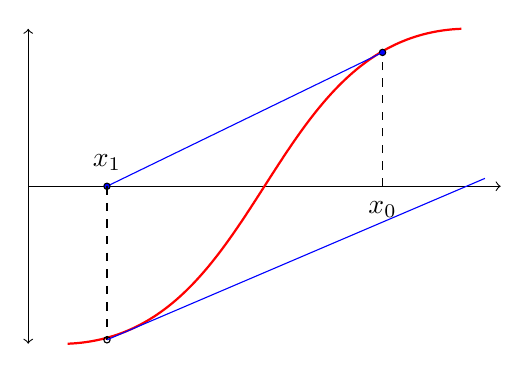
\begin{tikzpicture}%[decoration={
  %markings,% activar las marcas
  %mark= at position 2cm with{\arrow{stealth}}}]
		\draw [->] (0,0) -- (6,0);
		\draw [<->] (0,-2) -- (0,2);
		\draw [red, thick] (0.5,-2) .. controls (3,-1.9) and (3,1.9) .. (5.5,2);
		\draw (4.5,-0.3) node {$x_{0}$}; \pause
		\draw [dashed] (4.5,0) -- (4.5,1.69); \pause
		\draw [fill=blue] (4.5,1.7) circle (0.04); \pause
		\draw [blue, postaction={decorate}] (4.5,1.7) -- (1,0); \pause
		\draw (1,0.3) node {$x_{1}$}; \pause
		\draw [fill=blue] (1,0) circle (0.04);\pause
		\draw [dashed] (1,0) -- (1,-1.95); \pause
		\draw (1,-1.95) circle (0.04); \pause
		\draw [blue, postaction={decorate}] (1,-1.95) -- (5.8,0.1);
	\end{tikzpicture}
\end{center}
\end{frame}

\subsection{Ver. 1.0 algoritmo para el \texttt{MNR}}

\begin{frame}
\frametitle{Primera versión del algoritmo}
Esta versión del algoritmo del \funcionazul{MNR} requiere de un punto $x$ de aproximación a la raíz, así como la función $f$ y la derivada $df$ que se indican dentro del código.
\\
\bigskip
\pause
La versión 1.0 del \funcionazul{MNR} se debe de guardar en el módulo \funcionazul{moduloRaices}.
\end{frame}
\begin{frame}[fragile]
\frametitle{Primera versión del algoritmo}
\begin{lstlisting}[caption=Primera versión del MNR]
def newtonRaphson1(x, f, df, tol=1e-05):
    for i in range(50):
        dx = -f(x)/df(x)
        x = x + dx
        if abs(dx) < tol: return x, i
    print('Son demasiadas iteraciones\n')
\end{lstlisting}
\end{frame}
\begin{frame}
\frametitle{Ejercicio}
Con la versión 1.0 del \funcionazul{MNR} calcula la raíz positiva más pequeña de:
\begin{align*}
f (x) = x^{4} - 6.4 \, x^{3} + 6.45 \, x^{2} + 20.538 \, x - 31.752
\end{align*}
\pause
Tip: Para proporcionar el punto $x$ próximo a la función hay que graficar la misma, para que por inspección visual se indique el valor de $x$.
\end{frame}
\begin{frame}
\frametitle{Gráfica de la función $f (x)$}
\begin{figure}
    \centering
    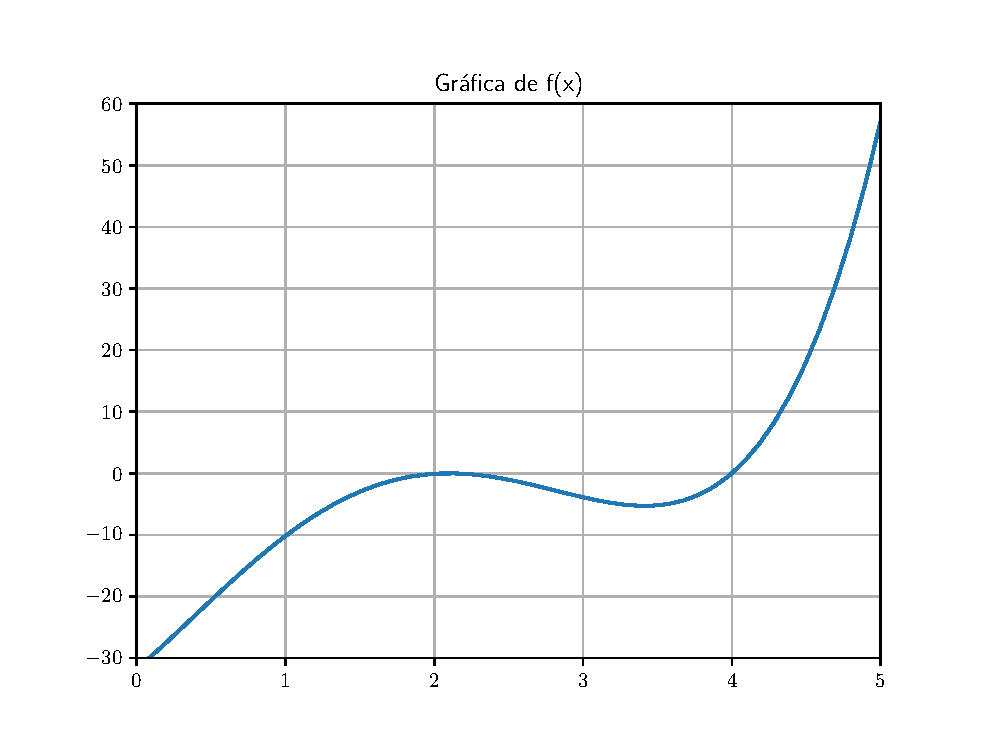
\includegraphics[scale=0.55]{Imagenes/raices_03_MNR_01.eps}
\end{figure}
\end{frame}
\begin{frame}
\frametitle{Eligiendo el punto $x$}
Revisando la gráfica anterior, con un acercamiento al trazo de la curva donde $y = 0$, \pause vemos que la raíz está cerca de $2.1$, \pause por lo que proponemos que $x = 2.0$
\end{frame}
\begin{frame}[allowframebreaks, fragile]
\frametitle{Código con la ver. 1.0}
\begin{lstlisting}[caption=Código para resolver el ejercicio 1]
from moduloRaices import newtonRaphson1
import numpy as np

def f(x): return x**4 - 6.4*x**3 + 6.45*x**2 + 20.538*x - 31.752
def df(x): return 4.0*x**3 - 19.2*x**2 + 12.9*x + 20.538

raiz, numIter = newtonRaphson1(2.0, f, df)

print('La raíz es = {0:1.5f}'.format(raiz))
print('Número de iteraciones realizadas = {0:}'.format(numIter))

x = np.linspace(0, 5)

# Aquí va la rutina de graficación
# No olvides llamar a las correspondientes librerías
\end{lstlisting}
\end{frame}
\begin{frame}
\frametitle{Gráfica con la raíz calculada}
\begin{figure}
    \centering
    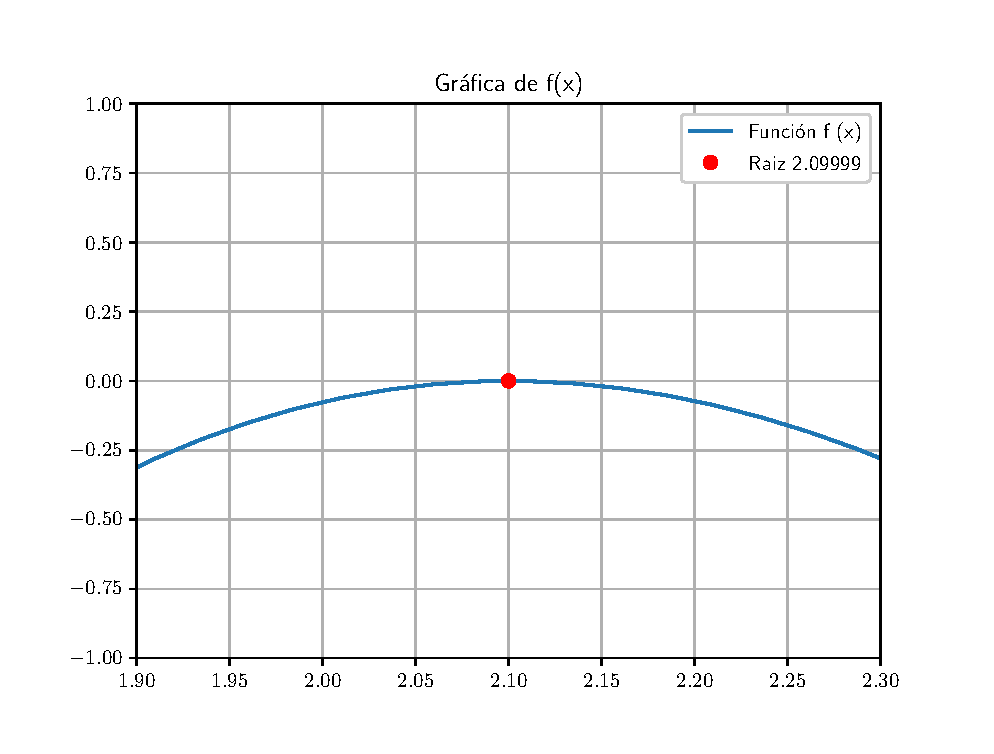
\includegraphics[scale=0.55]{Imagenes/raices_03_MNR_02.eps}
\end{figure}
\end{frame}
\begin{frame}
\frametitle{Error relativo}
Ocupando el valor exacto de la raíz: $2.1$, el error relativo ocupando el \funcionazul{MNR} es de $\num{4.7619d-6}$.
\end{frame}

\subsection{Ver. 2.0 del \texttt{MNR}}

\begin{frame}
\frametitle{Algoritmo para el \funcionazul{MNR}}
La siguiente versión del algoritmo para el \funcionazul{MNR} supone que la raíz a calcularse inicialmente está en el intervalo (a, b).
\end{frame}
\begin{frame}
\frametitle{Algoritmo para el \funcionazul{MNR}}
El punto medio del intervalo se utiliza como aproximación inicial de la raíz. \pause Los extremos del intervalo se actualizan luego de cada iteración.
\\
\bigskip
\pause
Si una iteración del \funcionazul{MNR} no se mantiene dentro del intervalo, se descarta y se reemplaza con el método de bisección.
\end{frame}
\begin{frame}
\frametitle{Algoritmo para el \funcionazul{MNR}}
Ya que el \funcionazul{MNR} requiere de la función $ f(x)$, así como su derivada, (denotadas por $f$ y $df$), \pause éstas deben ser proporcionadas por el usuario.
\\
\bigskip
\pause
La nueva versión debe de quedar dentro del \funcionazul{moduloRaices}.
\end{frame}
\begin{frame}[plain, allowframebreaks, fragile]
\frametitle{Algoritmo para el \funcionazul{MNR}}
\begin{lstlisting}[caption=Código para la segunda versión del MNR]
def newtonRaphson2(f, df, a, b, tol = 1.0e-9):
    fa = f(a)
    if fa == 0.0: return a

    fb = f(b)
    if f(b) == 0.0: return b

    if fa*fb > 0.0: print('La raiz no esta en el intervalo')
    x = 0.5 * (a + b)

    for i in range(30):
        fx = f(x)
        if abs(fx) < tol: return x

        if fa*fx < 0.0:
            b = x
        else:
            a = x; fa = fx

        dfx = df(x)
        
        try: dx = -fx/dfx
        except ZeroDivisionError: dx = b - a
        x =  x + dx
        
        # Si el resultado esta fuera del intervalo
        # se usa el metodo de biseccion
        if (b - x)*(x - a) < 0.0:
            dx = 0.5*(b-a)
            x = a + dx
        
        if abs(dx) < tol*max(abs(b), 1.0): return x
    
    print('Son demasiadas iteraciones')
\end{lstlisting}
\end{frame}
\begin{frame}
\frametitle{Ejercicio con la versión 2}
Usando la ver. 2.0 del algoritmo \funcionazul{MNR}, calcula las dos raíces de la función:
\begin{align*}
\sin \: x + 3 \: \cos \: x - 2 = 0
\end{align*}
en el intervalo $(-2, 2)$
\end{frame}
\begin{frame}
\frametitle{Primer paso: graficar la función}
La gráfica de la función en el intervalo dado es la siguiente:
\begin{figure}
	\centering
	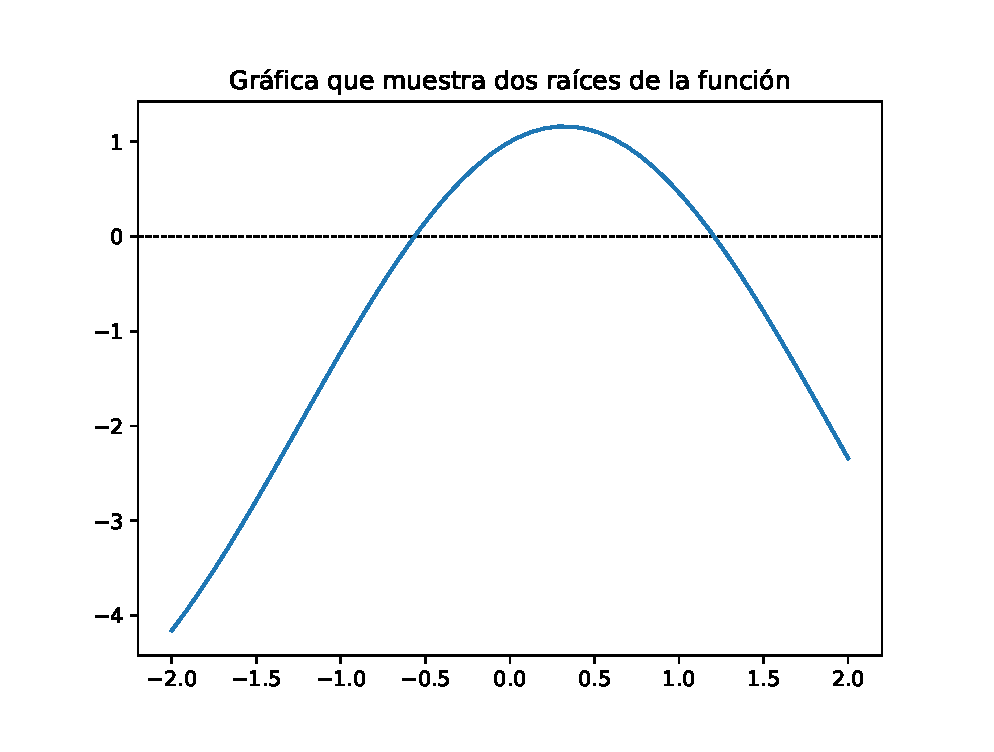
\includegraphics[scale=0.5]{Imagenes/Ejercicio_NR_Seno_01.eps}
\end{figure}
\end{frame}
\begin{frame}[fragile]
\frametitle{Intervalos de las raíces}
Con el método de incrementos sucesivos, estimamos cada intervalo donde se encuentran las raíces de la función.
\end{frame}
\begin{frame}[plain, fragile]
\frametitle{Intervalos de las raíces}
\begin{lstlisting}[caption=Intervalos para las raíces]
inicio, final, dx = -2., 2. , 0.01

a1, b1 = buscaraiz(f, inicio, final, 0.1)
print('Una raiz esta en el intervalo ({0:1.4f}, {1:1.4f})'.format(a1, b1))

inicio = b1

a2, b2 = buscaraiz(f, inicio, final, 0.1)
print('Otra raiz esta en el intervalo ({0:1.4f}, {1:1.4f})'.format(a1, b2))
\end{lstlisting}
\end{frame}
\begin{frame}[fragile]
\frametitle{Los intervalos}
El resultado que nos devuelve la función de incrementos sucesivos es:
\pause
\begin{verbatim}
Una raíz está en [ -0.6 , -0.5 ]
Una raíz está en [ 1.2 , 1.3 ]
\end{verbatim}
\end{frame}
\begin{frame}[allowframebreaks, plain, fragile]
\frametitle{Código completo}
\begin{lstlisting}[caption=Código completo para el ejercicio 1]
from ModuloRaices import buscaraiz, newtonRaphson
import matplotlib.pyplot as plt
import numpy as np


def f(x): return np.sin(x) + 3 * np.cos(x) - 2
def df(x): return np.cos(x) - 3 * np.sin(x)


intervalo1 = []
intervalo2 = []

inicio, final, dx = -2., 2. , 0.01


a1, b1 = buscaraiz(f, inicio, final, 0.1)
print('Una raiz esta en el intervalo ({0:1.4f}, {1:1.4f})'.format(a1, b1))
intervalo1.append(a1)
intervalo1.append(b1)

inicio = b1
a2, b2 = buscaraiz(f, inicio, final, 0.1)
print('Otra raiz esta en el intervalo ({0:1.4f}, {1:1.4f})'.format(a1, b2))
intervalo2.append(a2)
intervalo2.append(b2)

raiz1 = newtonRaphson(f, df, intervalo1[0], intervalo1[-1], 1.e-4)
print('La primera raiz en el intervalo ({0:1.4f}, {1:1.4f}) = '.format(intervalo1[0], intervalo1[-1], raiz1))

raiz2 = newtonRaphson(f, df, intervalo2[0], intervalo2[-1], 1.e-4)
print('La segunda raiz en el intervalo ({0:1.4f}, {1:1.4f}) = '.format(intervalo2[0], intervalo2[-1], raiz2))

x = np.linspace(-2,2)
plt.axhline(y=0, ls='dashed', lw=0.7, color='k')
plt.plot(x, f(x), color='g')
plt.plot(raiz1, 0, 'ro', label='Raiz 1 = ' + str(round(raiz1, 3)))
plt.plot(raiz2, 0, 'bo', label='Raiz 2 = ' + str(round(raiz2, 3)))
plt.legend(loc='lower right')
plt.title('Grafica que muestra dos raices de la funcion')
plt.show()
\end{lstlisting}    
\end{frame}
\begin{frame}
\frametitle{Solución}
La gráfica de la función en el intervalo dado es la siguiente:
\begin{figure}
	\centering
	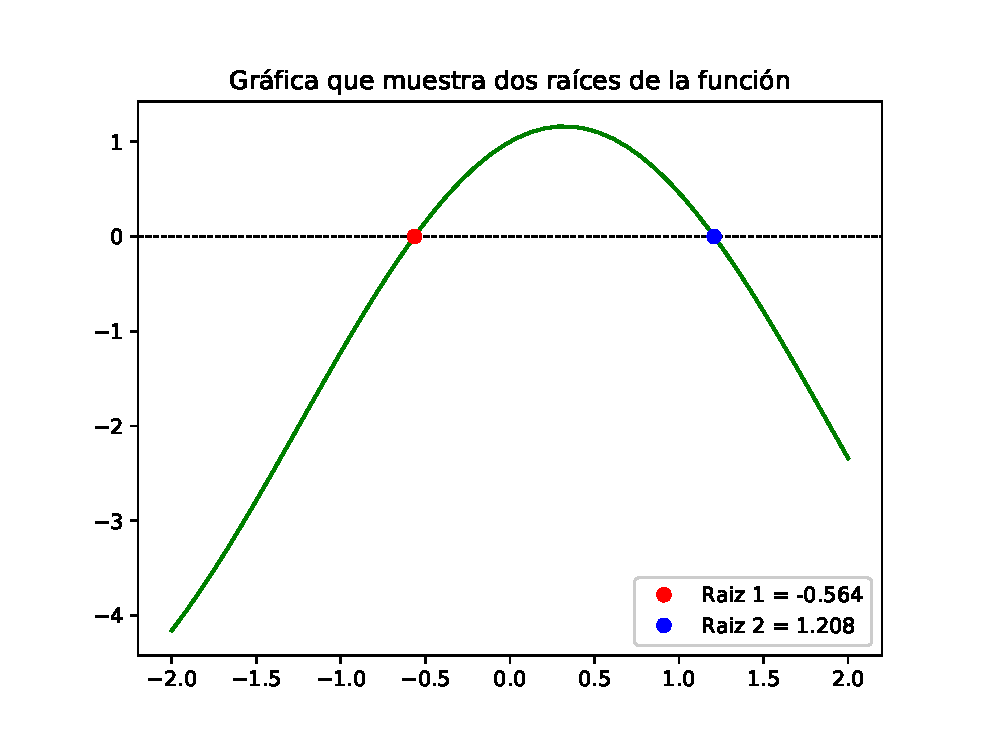
\includegraphics[scale=0.4]{Imagenes/Ejercicio_NR_Seno_02.eps}
	\caption{Implementando varias etapas, se calcularon las raíces de la función en el intervalo.}
\end{figure}
\end{frame}
% \begin{frame}
% \frametitle{Ejercicio}
% Encontrar la raíz positiva más pequeña de
% \[ f(x) = x^{4} - 6.4 \: x^{3} + 6.45 \: x^{2} + 20.538 \: x - 31.752\]
% Como en los ejercicios anteriores, es buena idea generar una gráfica de la función.
% \end{frame}
% \begin{frame}
% \frametitle{Gráfica del ejercicio}
% \begin{figure}
% 	\centering
% 	\visible<2-> {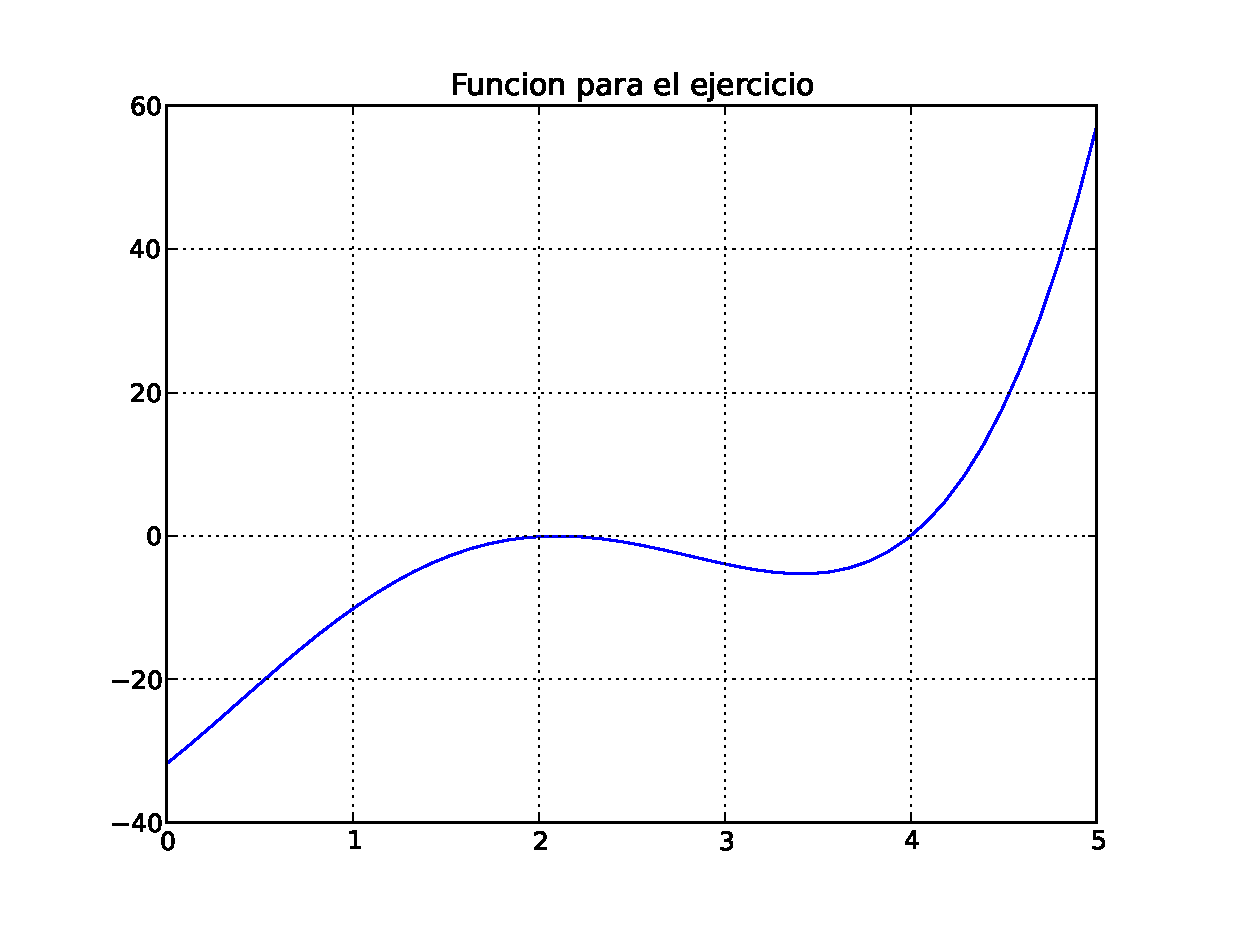
\includegraphics[scale=0.5]{Imagenes/raices08.eps}}
% \end{figure}
% \end{frame}
% \begin{frame}
% \frametitle{Caso particular para esta función}
% Al realizar un poco de álgebra, nos encontramos con lo siguiente:
% \[ 0.002 (x - 4.) (5. x + 9.) (10. x - 21.)^{2} \]
% La función tiene dos raíces reales y una de multiplicidad $2$.
% \end{frame}
% \begin{frame}
% \frametitle{Ajuste al código de NR}
% Como el método de NR se basa en detectar el cambio de signo en la función, en este caso, para una raíz con multiplicidad $2$, haremos un ajuste al código del método.
% \end{frame} 	
% \begin{frame}[allowframebreaks,plain, fragile]
% \frametitle{Ejercicio}
% \begin{lstlisting}[caption=Código para el ejercicio, style=FormattedNumber, basicstyle=\linespread{1.1}\ttfamily=\small, columns=fullflexible]
% def f(x): return x**4 - 6.4*x**3 + 6.45*x**2 + 20.538*x - 31.752
% def df(x): return 4.0*x**3 - 19.2*x**2 + 12.9*x + 20.538

% def newtonRaphson(x,tol=1e-09):
%     for i in range(30):
%         dx = -f(x)/df(x)
%         x = x + dx
%         if abs(dx) < tol: return x,i
%     print 'Son demasiadas iteraciones\n'

% raiz,numIter = newtonRaphson(2.0)

% print 'Raiz =',raiz
% print 'Numero de iteraciones =',numIter
% \end{lstlisting}
% \end{frame}
% \begin{frame}
% \frametitle{Convergencia del método}
% Se puede demostrar que la convergencia del método NR cerca de una raíz con multiplicidad es linear, más que cuadrática.
% \\
% \bigskip
% \pause
% La convergencia de una raíz múltiple se puede acelerar al cambiar la fórmula de NR.
% \end{frame}
% \begin{frame}
% \frametitle{Ajuste a la función NR}
% Se ajusta de la forma
% \[ x_{i + 1} = x_{i} - m \; \dfrac{f(x_{i})}{f^{\prime}(x_{i})} \]
% donde $m$ es la multiplicidad de la raíz (en el ejemplo, $m = 2$). Después de hacer los ajustes, el resultado se obtiene en $5$ iteraciones.
% \end{frame}
% \begin{frame}
% \frametitle{Solución del ejercicio}
% \begin{figure}
% 	\centering
% 	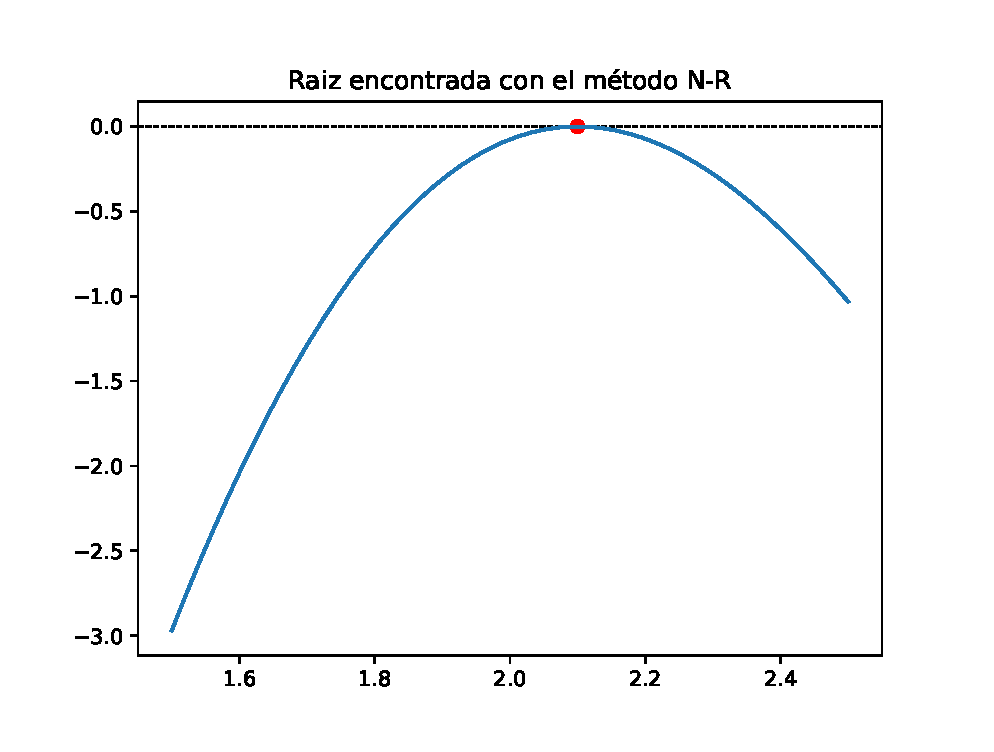
\includegraphics[scale=0.5]{Imagenes/Raiz_NR_02.eps}
% \end{figure}
% \end{frame}
% %\begin{frame}
% % \frametitle{Ejercicios}
% % \begin{enumerate}
% % \item Encuentra las raíces de $x \sin x + 3 \cos x - x = 0$ en el intervalo $(-6,6)$ \\
% % \item Calcula todas las raíces reales de $x^{4} + 0.9x^{3} - 2.3x^{2} + 3.6x - 25.2 = 0$. \\
% % \item Calcula todas las raíces reales de $x^{4} + 2x^{3} - 7x^{2} + 3 = 0$. \\
% % \item Calcula todas las raíces de $\sin x - 0.1x = 0$.
% % \end{enumerate}
% % \end{frame}
% \subsection{Método de la falsa posición}
% \begin{frame}
% \frametitle{Método de la falsa posición}
% Este método es parecido al de bisección, ya que el intervalo que contiene a la raíz se va reduciendo.
% \\
% \bigskip
% En vez de bisectar de manera monótona el intervalo, se utiliza una interpolación lineal ajustada a dos puntos extremos para encontrar la aproximación de la raíz.
% \end{frame}
% \begin{frame}
% La función está bien aproximada por la interpolación lineal, con lo que las raíces tendrán una buena precisión; la iteración convergerá más rápido que como ocurre con el método de bisección.
% \end{frame}
% \begin{frame}
% Dado un intervalo $[a,c]$ que contenga a la raíz, la función lineal que pasa por $(a,f(a))$ y $(c,f(c))$ se escribe como:
% \[ y = f(a) + \dfrac{f(c) - f(a)}{c - a} \: (x - a) \]
% de donde se despeja $x$:
% \[ x = a + \dfrac{c - a}{f(c) - f(a)} \: \big[ y - f(a)\big] \]
% \end{frame}
% \begin{frame}
% La coordenada $x$ en donde la línea intersecta al eje $x$ se determina al hacer $y=0$ en la ecuación anterior, por tanto:
% \[ b = a - \dfrac{c - a}{f(c) - f(a)} \: f(a) = \dfrac{a \: f(c) - c \: f(a)}{f(c)-f(a)} \]
% Después de encontrar $b$, el intervalo $[a, c]$ se divide en $[a, b]$ y $[b, c]$.
% \end{frame}
% \begin{frame}
% Si $f(a) \: f(b) \leq 0$, la raíz se encuentra en $[a, b]$; en caso contrario, está en $[b, c]$. 
% \\
% \bigskip
% Los extremos del nuevo intervalo que contiene a la raíz se renombran para el siguiente paso como $a$ y $c$.
% \\
% \bigskip
% El procedimiento de interpolación se repite hasta que las raíces estimadas convergen.
% \end{frame}
% \begin{frame}[fragile]
% \frametitle{Método de la falsa posición}
% \begin{center}
% 	\begin{tikzpicture}[font=\small]
% 		\draw [->] (0,0) -- (7,0);
% 		\draw [<->](0,-3) -- (0,3);
% 		\draw [red, thick] (1,3) .. controls (1.5,0.5) and (5,-2) .. (6.5,-2);
% 		\draw (1,-0.3) node {$a$};
% 		\draw (0.7, 2.4) node {$f(a)$};
% 		\draw (6,0.3) node {$c$};
% 		\draw (6.3, -2.4) node {$f(c)$};
% 		\draw [dashed] (1.2,0) -- (1.2,2.35);
% 		\draw [dashed] (6.3,0) -- (6.3,-1.98);\pause
% 		\draw (1.2,2.35) -- (6.3,-1.98);
% 		\draw  (3,3) node {1a. interpolación};
% 		\draw [->] (3,2.6) -- (2,2);\pause
% 		\draw  (5,1) node {1a. aproximación};
% 		\draw [->] (5,0.6) -- (4.1,0.1);
% 		\draw (4,0.3) node {$b_{1}$};
% 		\draw (4, -1.3) node {$f(b_{1})$};
% 		\draw [dashed] (4,0) -- (4,-0.9);
% 	\end{tikzpicture}
% \end{center}
% \end{frame}
% \begin{frame}[fragile]
% \frametitle{Método de la falsa posición}
% \begin{figure}
% 	\centering
% 	\begin{tikzpicture}[font=\small]
% 		\draw [->] (0,0) -- (7,0);
% 		\draw [<->] (0,-3) -- (0,3);
% 		\draw [red, thick] (1,3) .. controls (1.5,0.5) and (5,-2) .. (6.5,-2);
% 		\draw (1,-0.3) node {$a$};
% 		\draw (0.7, 2.4) node {$f(a)$};
% 		\draw (4,0.3) node {$c$};
% 		\draw (4, -1.3) node {$f(c)$};
% 		\draw [dashed] (4,0) -- (4,-0.9);
% 		\draw [dashed] (1.2,0) -- (1.2,2.35);\pause
% 		\draw (1.2,2.35) -- (4,-0.9);
% 		\draw  (4,2) node {2a. interpolación};
% 		\draw [->] (4,1.6) -- (2.5,1);\pause
% 		\draw [dashed] (3.25,0) -- (3.25,-0.43);
% 		\draw (3.2, 0.3) node {$b_{2}$};
% 		\draw (3, -0.75) node {$f(b_{2})$};
% 		\draw  (6,1) node {2a. aproximación};
% 		\draw [->] (5.5,0.8) -- (3.3,0.1);
% 	\end{tikzpicture}
% 	\caption{Se renombran los extremos y se realiza la segunda aproximación lineal.}
% \end{figure}
% \end{frame}
% \begin{frame}
% \textcolor{red}{La desventaja de este método es que aparecen extremos fijos}: uno de los extremos de la sucesión de intervalos no se mueve del punto original, por lo que las aproximaciones a la raíz, denotadas por $b_{1}$, $b_{2}$, $b_{3}$, etc. convergen a la raíz exacta solamente por un lado.
% \end{frame}
% \begin{frame}
% Los extremos fijos no son deseables debido a que hacen más lenta la convergencia, en particular cuando el intervalo es grande o cuando la función se desvía de manera significativa de una línea recta en el intervalo.
% \\
% \bigskip
% ¿Qué podemos hacer al respecto?
% \end{frame}
% \subsection{Método de la falsa posición modificado}
% \begin{frame}
% \frametitle{Método de la falsa posición modificado}
% En este método, el valor de $f$ en un punto fijo se divide a la mitad si este punto se ha repetido más de dos veces.
% \\
% \bigskip
% El extremo que se repite se llama extremo fijo. La excepción para esta regla es que para $i = 2$, el valor de $f$ en un extremo se divide entre $2$ de inmediato si no se mueve.
% \end{frame}
% \begin{frame}[fragile]
% \frametitle{Método de falsa posición modificado}
% \begin{figure}
% 	\centering
% 	\begin{tikzpicture}[font=\small]
% 		\draw [->] (0,0) -- (7,0);
% 		\draw [<->](0,-3) -- (0,3);
% 		\draw [red, thick] (1,3) .. controls (1.5,0.5) and (5,-2) .. (6.5,-2);
% 		\draw (1,-0.3) node {$a$};
% 		\draw (0.7, 2.4) node {$f(a)$};
% 		\draw (6,0.3) node {$c$};
% 		\draw (6.3, -2.4) node {$f(c)$};
% 		\draw [dashed] (1.2,0) -- (1.2,2.35);
% 		\draw [dashed] (6.3,0) -- (6.3,-1.98);\pause
		
% 		\draw (1.2,2.35) -- (6.3,-1.98);
% 		\draw  (3,3) node {1a. interpolación};
% 		\draw [->] (3,2.6) -- (2,2);\pause
% 		\draw  (5,1) node {1a. aproximación};
% 		\draw [->] (5,0.6) -- (4.1,0.1);
% 		\draw (4,0.3) node {$b_{1}$};
% 		\draw (4, -1.3) node {$f(b_{1})$};
% 		\draw [dashed] (4,0) -- (4,-0.9);

% 	\end{tikzpicture}
% \end{figure}
% \end{frame}
% \begin{frame}[fragile]
% \frametitle{Método de la falsa posición modificado}
% \begin{figure}
% 	\centering
% 	\begin{tikzpicture}[font=\small]
% 		\draw [->] (0,0) -- (7,0);
% 		\draw [<->] (0,-3) -- (0,3);
% 		\draw [red, thick] (1,3) .. controls (1.5,0.5) and (5,-2) .. (6.5,-2);
% 		\draw (1,-0.3) node {$a$};
% 		\draw (0.7, 2.4) node {$f(a)$};
% 		\draw (4,0.3) node {$c$};
% 		\draw (4, -1.3) node {$f(c)$};
% 		\draw [dashed] (4,0) -- (4,-0.9);
% 		\draw [dashed] (1.2,0) -- (1.2,2.35);\pause
% 		\draw  (4,2) node {2a. interpolación};
% 		\draw [->] (4,1.6) -- (1.8,1);
% 		\draw (1.2,1.3) -- (4,-0.9);
% 		\draw (0.8, 1.3) node {$\frac{f(a)}{2}$};
% 		\pause
% 		\draw [dashed] (3.25,0) -- (3.25,-0.43);
% 		\draw (3.2, 0.3) node {$b_{2}$};
% 		\draw (3, -0.75) node {$f(b_{2})$};
% 		\draw  (6,1) node {2a. aproximación};
% 		\draw [->] (5.5,0.8) -- (3.3,0.1);
% 	\end{tikzpicture}
% 	\caption{Se evitan los extremos fijos de tal manera que se acelera la convergencia.}
% \end{figure}
% \end{frame}
% \subsection{Método de la secante}
% \begin{frame}
% \frametitle{Método de la secante}
% A diferencia del método de Newton, el valor de $f^{\prime}$ se aproxima utilizando dos valores de iteraciones consecutivas de $f$.
% \\
% \bigskip
% Con lo que se elimina la necesidad de evaluar tanto a $f$ como a $f^{\prime}$ en cada iteración.
% \end{frame}
% \begin{frame}
% Las aproximaciones sucesivas para la raíz en el método de la secante están dadas por:
% \[ x_{n} = x_{n - 1} - y_{n - 1} \dfrac{x_{n - 1} - x_{n - 2}}{y_{n - 1}- y_{n - 2}}, \hspace{1cm} n = 2,3,\ldots \]
% donde $x_{0}$ y $x_{1}$ son dos suposiciones iniciales para comenzar la iteración.
% \end{frame}
% \begin{frame}[fragile]
% \frametitle{Método de la secante}
% \setbeamercovered{invisible}
% \begin{center}
% 	\begin{tikzpicture}[font=\small]
% 		\draw [->] (0,0) -- (7.5,0);
% 		\draw [->] (0,0) -- (0,4);
% 		\draw [red, thick](7,3.5) .. controls (6.3,2) and (4.5,0.3) .. (1,0);
% 		\draw [dashed] (6.8,3.1) -- (6.8,0);
% 		\draw (6.6,-0.3) node {$x_{0}$};
% 		\draw (6.6, 3.3) node {$f_{0}$};
% 		\draw [dashed] (5.5,1.65) -- (5.5,0);
% 		\draw (5.25,-0.3) node {$x_{1}$};
% 		\draw (5.25, 1.8) node {$f_{1}$};
% 		\draw (6.8,3.1) -- (4.1,0);\pause
% 		\draw (4,-0.3) node {$x_{2}$};
% 		\draw [dashed] (4.1,0) -- (4.1,0.8);
% 		\draw (3.9, 1) node {$f_{2}$};\pause
% 		\draw (5.5,1.65) -- (2.9,0);
% 		\draw (2.8,-0.3) node {$x_{3}$};
% 	\end{tikzpicture}
% \end{center}
% \end{frame}
% \begin{frame}
% \frametitle{Atento aviso}
% En las técnicas de falsa posición, falsa posición modificada y el método de la secante, no hemos presentado como tal un código en \python{} que nos devuelva las raíces, por lo que tendrás que proponer un código para cada una de las técnicas.
% \\
% \medskip
% Ese código lo vas a utilizar par resolver los problmeas y ejercicios del examen.
% \end{frame}

\end{document}